\begin{algorithm}[h]
\caption{\small Compresión continua de KV cache (CKV) con InfiniPot-V}
\label{alg:infinipot_v_main}
\footnotesize
\begin{algorithmic}[0]
\Require Memory budget $|M|$, target cache size $|C|$, TaR ratio $\alpha$
\State Initialize $K, V \gets \emptyset$ \Comment{Empty KV cache}
\While{el flujo de video continúa}
    \State (1) Process: $K_{\text{new}}, V_{\text{new}} \gets \text{Process new frame}$; $K \gets [K; K_{\text{new}}]$, $V \gets [V; V_{\text{new}}]$ \Comment{Append new tokens}
    \If{$\text{len}(K) \geq |M|$} \Comment{Memory budget exceeded}
        \State (2) Extract: $K_{\text{recent}}, V_{\text{recent}} \gets \text{los }r\text{ frames más recientes de }K, V$ \Comment{$\text{len}(K) = \text{len}(V) = |M|$}
        \State (3) TaR: $s^{\text{TaR}} \gets \text{ComputeTaRScores}(K)$; $\mathcal{I}_{\text{TaR}} \gets \text{TopK}(s^{\text{TaR}}, \alpha|C| - \text{len}(K_{\text{recent}}))$ \Comment{Sec.~\ref{subsec:tar}}
        \State (4) VaN: $s^{\text{VaN}} \gets \text{ComputeAdaptiveVaNScores}(V)$; $\mathcal{I}_{\text{VaN}} \gets \text{TopK}(s^{\text{VaN}}, (1-\alpha)|C|)$ \Comment{Sec.~\ref{subsec:van}}
        \State (5) Combine: $\mathcal{I} \gets \mathcal{I}_{\text{TaR}} \cup \mathcal{I}_{\text{VaN}} \cup \text{Indices}(K_{\text{recent}})$; $K \gets K[\mathcal{I}]$, $V \gets V[\mathcal{I}]$ \Comment{Compress to $|C|$ size}
    \EndIf
    \If{user query arrives} \State Generate response using current $K, V$ \EndIf
\EndWhile
\end{algorithmic}
\end{algorithm}

\section{InfiniPot-V: Memory-Constrained Streaming Video Understanding}
\label{sec:method}

\begin{figure*}[t!]
\centerline{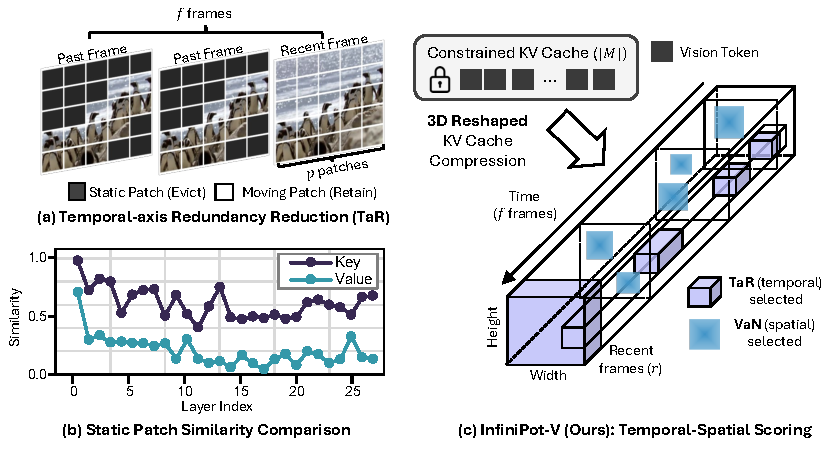
\includegraphics[width=0.9\textwidth]{Figures/fig2.pdf}}
\caption{\textbf{Compresión espaciotemporal de KV cache (TaR y VaN).} (a) Redundancia temporal entre frames adyacentes, mostrando patches estáticos que pueden desalojarse de frames pasados; (b) similitud coseno por capa de embeddings Key/Value para patches estáticos entre frames consecutivos en \texttt{LLaVA-Next-Video-7B}; (c) InfiniPot-V realiza compresión espaciotemporal query-agnostic, reduciendo la redundancia temporal con TaR y seleccionando tokens mediante puntuación espacial VaN.}
\vspace{-0.1in}
\label{fig:cache_compression}
\end{figure*}

Presentamos \textbf{InfiniPot-V}, un framework CKV diseñado para SVU con restricciones de memoria. Como se muestra en la Fig.~\ref{fig:background}(d) y en el Algoritmo~\ref{alg:infinipot_v_main}, InfiniPot-V procesa flujos de video aplicando compresión continua de KV cache dentro de un presupuesto de memoria fijo. 
En este framework, los KV embeddings de los frames entrantes se almacenan hasta alcanzar el límite de memoria $|M|$. En ese punto, la compresión reduce la cache a un tamaño objetivo menor $|C|$ ($|M| \gg |C|$), reteniendo solo los vision tokens más esenciales según dos criterios. El espacio liberado ($|M| - |C|$) permite acomodar nuevos frames. Este proceso se repite continuamente, permitiendo un procesamiento eficiente del stream bajo restricciones estrictas de memoria. Cuando se emite una user query, el modelo responde usando la cache comprimida que resume el contexto visual de todos los frames previos. Notablemente, la compresión añade solo un 0.5\% de overhead respecto al tiempo de procesamiento de los frames de entrada.

InfiniPot-V aprovecha dos criterios de desalojo de tokens: \textit{Temporal-axis Redundancy (TaR)} y \textit{Value Norm (VaN)} para identificar tokens cruciales al comprimir la KV cache. En las siguientes subsecciones detallamos cada criterio y, finalmente, describimos cómo combinarlos de forma efectiva.

\subsection{Temporal-axis Redundancy (TaR) Reduction via Patch-wise Similarity}\label{subsec:tar}

Video streams exhibit inherent spatiotemporal redundancy across frames~\cite{h264,shen2024longvu,tao2024dycokedynamiccompressiontokens}.
In this section, we focus on exploiting temporal redundancy, as illustrated in Fig.~\ref{fig:cache_compression}(a) where static patches\footnote{In MLLMs, each vision patch corresponds to a single token, so we use these terms interchangeably.} (e.g., background) persist across frames. For MLLMs processing videos with fixed memory usage, identifying this redundancy in KV caches is crucial. Our analysis in Fig.~\ref{fig:cache_compression}(b) reveals that Key embeddings effectively capture temporal redundancy, exhibiting higher cosine similarity for static patches between adjacent frames compared to Value embeddings, across all layers.

Building on this insight, we propose TaR, a technique that performs a patch-wise comparison of Key embeddings along the temporal axis to detect and reduce redundant tokens. As shown in Fig.~\ref{fig:cache_compression}(c), we introduce a 3D reshaping of Key embeddings to enable direct comparison of corresponding patches across frames. Based on this structured KV cache, the TaR implementation starts with a memory constraint of $|M|$ tokens, processing $f$ consecutive video frames, each containing $p = |M|/f$ vision tokens. To maintain temporal continuity, we designate the $r$ latest frames as \textit{recent frames} and retain them in full. The older \textit{past frames} ($f-r$ frames) are selectively compressed based on their patch-wise similarity to recent frames.

To measure the patch-wise similarity between frames, we divide the current Key embeddings $K \in \mathbb{R}^{H \times (f\times p) \times D}$ into $K_{\text{recent}} \in \mathbb{R}^{H \times r \times p \times D}$ and $K_{\text{past}} \in \mathbb{R}^{H \times (f - r) \times p \times D}$, representing the recent and past frames respectively. For each spatial coordinate $(i, j)$, we compute the $\ell_2$-normalized cosine similarity between recent and past frames of the same patch coordinate:
% \vspace{-.1in}
\begin{equation}\label{eq:tar}
s^{\text{TaR}}(t, i, j) = - \frac{1}{r} \sum_{t'=1}^{r} \text{cos}\Big( K_{\text{past}}^{(t,i,j)}, K_{\text{recent}}^{(t', i, j)} \Big).
\end{equation}
Here, $s^{\text{TaR}}(t, i, j)$ is the importance score of the patch in $t$-th frame at $(i,j)$ coordinate.
The negative sign is applied so that a higher computed score indicates lower redundancy (i.e., the token is more distinctive).
This ensures that tokens with less temporal similarity to recent frames are prioritized.
We then select the least redundant tokens (i.e., higher score) in past frames using the Top-K operator:
\begin{equation}
\mathcal{I_\text{{TaR}}} = \text{TopK}(s^{\text{TaR}}, |C| - |K_{\text{recent}}|),
\end{equation}
where $|C|$ is the target cache compression size and $|K_{\text{recent}}|=rp$ accounts for the recent frame tokens that are always retained.
The compressed key-value pairs are formed by concatenating the selected key frame tokens with all recent frame tokens:
\begin{equation}
\tilde{K}_{\text{TaR}} = \text{Concat}\big(K[:, \mathcal{I_\text{{TaR}}}, :],K_{\text{recent}}\big), \qquad
\tilde{V}_{\text{TaR}} = \text{Concat}\big(V[:, \mathcal{I_\text{{TaR}}}, :],V_{\text{recent}}\big).
\end{equation}
By fully preserving the most recent frames, we maintain complete information on rapidly changing or newly introduced content, while selectively retaining distinctive visual elements from the past.

\subsection{Spatial Semantic Importance Preserving with Value Norm (VaN)}\label{subsec:van}

\begin{wrapfigure}{t}{0.5\columnwidth}
\centerline{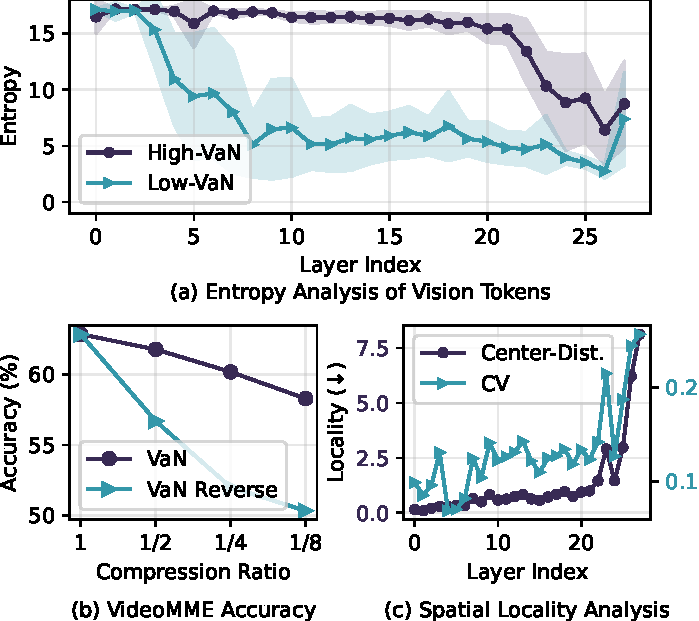
\includegraphics[width=0.5\columnwidth]{Figures/fig3.pdf}}
\caption{\textbf{Value Norm (VaN) Analysis.} (a) Entropy analysis of vision token representations grouped by their VaN scores. (b) VideoMME performance under varying cache compression ratios using either VaN or reverse-VaN for token selection. (c) Layer-wise locality of VaN, measured by center distance and coefficient of variation (CV); lower values indicate stronger spatial consistency. \texttt{LLaVA-Next-7B} with Video-MME used.}\label{fig:entropy}
\vspace{-.2in}
\end{wrapfigure}

While TaR focuses on reducing temporal redundancy, VaN serves a complementary role: identifying and preserving semantically salient regions within each video frame, independent of the query.
To achieve this, we employ Value embeddings ($V$), which inherently capture semantic information in transformer attention~\cite{NIPS2017_3f5ee243}.
Specifically, we introduce Value Norm (VaN) as a metric for token-level semantic importance: $s^{\text{VaN}} = \|V^{(t,i,j)}\|_2$.

\paragraph{Analysis of Value Norm.}
We hypothesize that tokens with higher VaN contain richer semantic information, making them more valuable for video understanding.
To quantify semantic importance, we project vision token representations from each layer into the vocabulary space~\cite{neo2025towards} and compute the entropy of the resulting word probability distribution, where the higher entropy implies greater informativeness~\cite{farquhar2024detecting,chan2025analyzing}.
As shown in Fig.~\ref{fig:entropy} (a), tokens with higher VaN consistently exhibit higher entropy, confirming their semantic significance.
This advantage translates to improved performance: Fig.~\ref{fig:entropy}~(b) shows that retaining high-VaN tokens achieves substantially higher video understanding accuracy across various compression ratios compared to low-VaN (VaN Reverse) tokens.


\paragraph{Layer-wise Adaptive Pooling.}
An analysis of VaN distributions reveals strong spatial locality patterns in early to middle layers, which gradually diminish in deeper layers as shown in Fig.~\ref{fig:entropy}(c). To measure spatial locality patterns across layers, we employ two methods: (1) compute the average distance between the center point and surrounding points within a $3\times3$ window spanning the VaN values of each frame (center-dist.), and (2) measure the Coefficient of Variance (CV) to quantify dispersion of VaN distributions. Lower values in both metrics—smaller center-dist. and CV—indicate that VaN scores are closely clustered, implying high spatial locality, whereas higher values reflect greater dispersion and lower locality.

As shown in Fig.~\ref{fig:entropy}~(c), both metrics consistently indicate strong locality in early to middle layers, while gradually diminishing in deeper layers. Based on this observation, we design an adaptive spatial pooling mechanism that adjusts the average pooling kernel size per layer. To implement this, we design a mapping function $g$ that assigns kernel sizes in inverse relation to each layer's CV: 
$$ 
\mathrm{PoolSize}(CV_l) = g(CV_l) \quad \text{where} \quad g : \mathbb{R}^+ \rightarrow {1,3,5,7} 
$$ 
This approach assigns larger pooling kernels (e.g., 7) to lower layers with smaller CV values (higher spatial locality), and smaller kernels (e.g., 1, implying no pooling) to upper layers with larger CV values, thus preserving fine-grained details where needed.

For KV cache compression, we select tokens using VaN scores processed through our adaptive pooling mechanism, retaining the Top-$|C|$ tokens with highest pooled VaN values as described in Fig.~\ref{fig:cache_compression}(c): $I_\text{{VaN}} = \text{TopK}(\text{VaN}_{\text{pool}}, |C|)$
\begin{equation}
\tilde{K}_{\text{VaN}} = K[:, \mathcal{I_\text{{VaN}}}, :], \quad \tilde{V}_{\text{VaN}} = V[:, \mathcal{I_\text{{VaN}}}, :].
\end{equation}


\begin{table}[t]
\small
  \centering
  \label{tab:video_qa_comparison}
  \begin{tabular}{l c c c c c c c}
    \toprule
    \textbf{Method}                 & \textbf{Size} & \textbf{\# Frames} & \textbf{Budget} & \textbf{EgoSchema} & \textbf{MLVU} & \textbf{VideoMME} & \textbf{LVB} \\
    Max Duration               &               &                    &             \textbf{$|M|$}    & 3\,min           & 120\,min           & 60\,min          & 60\,min     \\
    \midrule
    GPT4-V*                         & –             & 1fps              & –                       & 55.6               & –            & 60.7              & –           \\
    GPT4-o*                         & –             & 1fps              & –                       & 72.2               & 66.2         & 77.2              & 66.7        \\ \midrule
    % Gemini-2.5 Pro*                 & –             & –                  & –                       & –                  & –            & 84.8              & –           \\
    % Video-LLaVA*                    & 7B           & 8                  & 4K                     & 38.4               & 47.3         & 40.4              & 37.6        \\
    LLaVA-OV*                       & 7B           & 32                 & 8K                     & 60.1               & 64.7         & 58.2              & –           \\
    LongVU*                         & 7B           & 1fps              & 8K                     & 67.6               & 65.4         & 60.6              & –           \\
    LongVU*             & 3B           & 1fps              & 8K                     & 59.1               & 55.9         & 51.5              & –           \\
    \midrule
    Qwen-2-VL                       & 7B           & 768                & 50K                    & 65.2              & 65.8        & 63.9             & 58.8       \\
\mscellt Qwen-2-VL + \textbf{Ours}                & 7B           & 768                & 6K                     & 65.6                  & 65.8        & 62.8             & 58.4       \\
    LLaVA-Next                      & 7B           & 128                & 25K                    & 67.6               & 68.7        & 62.8             & 63.5       \\
\mscellt    LLaVA-Next + \textbf{Ours}               & 7B           & 128                & 6K                     & 65.8                  & 65.2        & 61.1             & 60.9       \\
    Qwen-2.5-VL                     & 3B           & 768                & 50K                    & 64.4               & 63.3        & 60.3             & 59.9       \\
\mscellt Qwen-2.5-VL + \textbf{Ours}                & 3B           & 768                & 6K                     & 61.8                   & 62.1        & 59.3             & 56.5       \\
    \bottomrule
  \end{tabular}
  \vspace{2mm}
    \caption{Comparación de la exactitud de varios MLLMs en cuatro benchmarks de Offline Video Understanding (OVU). * denota cifras tomadas del artículo oficial.}
   \label{tab:open-source}
   % \vspace{-.2in}
\end{table}

\begin{table}[t]
\small
  \centering
  \begin{tabular}{lccccccccc}
    \toprule
    \textbf{Compression} & \textbf{Budget} & \multicolumn{3}{c}{\textbf{Video MME}} & \multicolumn{3}{c}{\textbf{MLVU}} & \\
    \cmidrule(lr){3-5} \cmidrule(lr){6-8}
    \textbf{Method} & \textbf{$|M|$} & \textbf{Short} & \textbf{Med} & \textbf{Long} & \textbf{Holistic} & \textbf{Single} & \textbf{Multi} & \textbf{Avg}. \\
    \midrule
    FullKV & 50K & 74.7 & 62.1 & 55.0 & 76.3 & 73.9 & 43.3 & 64.2 \\
    \midrule
    TTC~\cite{tao2024dycokedynamiccompressiontokens} & 3K & 66.8 & 51.2 & 47.9 & 72.1 & 58.8 & 33.2 & 54.8 \\
    (IVC) & 6K & 72.6 & 55.0 & 51.7 & 76.3 & 60.9 & 36.7 & 58.4 \\
    \midrule
    STC~\cite{shen2024longvu} & 3K & 67.9 & 51.0 & 49.3 & 71.5 & 58.6 & 33.9 & 55.0 \\
    (IVC) & 6K & 72.6 & 56.2 & 51.6 & 74.3 & 61.1 & 35.9 & 57.9 \\
    \midrule
    \mscells \textbf{InfiniPot-V} & 3K & 73.9 & 57.8 & 51.8 & 77.7 & 70.4 & 43.2 & 63.1 \\
    \mscellt (CKV) & 6K & 74.1 & 60.8 & 53.4 & 77.2 & 72.3 & 44.8 & 64.3 \\
    \bottomrule
\end{tabular}
\vspace{2mm}
  \caption{Comparison under memory-constrained settings (3, 6K memory-budget) with Input Video Compression (IVC) methods: TTC from DyCoke~\cite{tao2024dycokedynamiccompressiontokens} and STC from LongVU~\cite{shen2024longvu}. \texttt{Qwen-2-VL-7B} used across VIdeoMME and MLVU benchmarks. Results comparing memory-unconstrained IVC methods (without KV cache compression) with InfiniPot-V are provided in Tab.~\ref{tab:full_ivc}.} 
  \label{tab:ic_cache}
% \vspace{-4mm}
\end{table}



\subsection{Design Space Exploration}
\label{subsec:combine}

\textbf{Combining TaR and VaN for Token Selection.}
TaR and VaN capture complementary aspects of spatio-temporal redundancy in streaming video. To integrate them, we prioritize TaR-based selection by first allocating $\alpha |C|$ tokens to TaR, then filling the remaining $(1 - \alpha)|C|$ with VaN-selected tokens. This two-stage selection strategy effectively balances temporal and feature importance. A detailed hyperparameter exploration, including sweeps over $\alpha$ and the size of the recent frame window $r$, is provided in Appendix.~\ref{appn:hyper_parameter}.


\textbf{Comparison with Memory-Constrained Alternatives.}
A natural question is whether IVC or KVC can be adapted for SVU under memory constraints. To explore this, we apply query-agnostic methods such as spatial token compression (STC) and token temporal merging (TTC) from LongVU~\cite{shen2024longvu} and DyCoke~\cite{tao2024dycokedynamiccompressiontokens}. InfiniPot-V outperforms all these baselines by a notable accuracy margin, demonstrating the strength of continual compression over expressive key-value embeddings (details in Tab.~\ref{tab:ic_cache}). 
